\documentclass[border=2pt]{standalone}
\usepackage{tikz}
\usetikzlibrary{calc} \usetikzlibrary{positioning} \usetikzlibrary{shapes,arrows} \usetikzlibrary{plotmarks}
\usepackage{pgfplots}
\usetikzlibrary{patterns}

\begin{document}

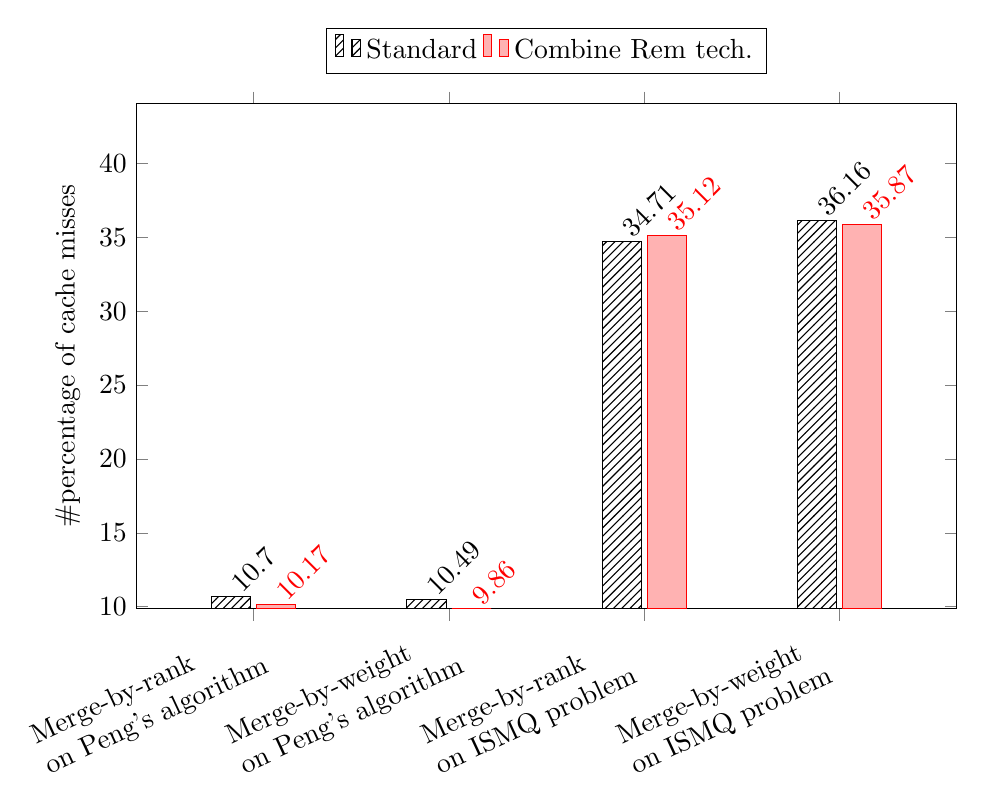
\begin{tikzpicture}
  \centering
  \begin{axis}[
  	bar width=0.5cm,
    ybar,
    xtick=\empty,
    enlargelimits=0.20,
    legend style={at={(0.5,1.15)},
    anchor=north,legend columns=-2},
    ylabel={\#percentage of cache misses},
    symbolic x coords={VGLCS Rank,VGLCS Weight, ISMQ Rank, ISMQ Weight},
    xtick={VGLCS Rank,VGLCS Weight, ISMQ Rank, ISMQ Weight},
    height=8cm,width=12cm,
    nodes near coords,
    nodes near coords align={vertical},
    every node near coord/.append style={
        anchor=mid west,
        rotate=45
    },
    xticklabel style={
	    inner sep=0pt,
	    anchor=north east,
	    rotate=25,
	    % font=\scshape,
        text width=9em
    },
    enlarge y limits={upper,value=0.3},
    xticklabels={
        Merge-by-rank \\on Peng's algorithm,
        Merge-by-weight \\on Peng's algorithm,
        Merge-by-rank \\on ISMQ problem,
        Merge-by-weight \\on ISMQ problem,
    },
    ]
    \addplot[pattern=north east lines] coordinates 
    	{(VGLCS Rank,10.701) (VGLCS Weight,10.491)
    	 (ISMQ Rank,34.713) (ISMQ Weight,36.162)
    	};
    \addplot coordinates 
    	{(VGLCS Rank,10.167) (VGLCS Weight,9.856)
    	 (ISMQ Rank,35.122) (ISMQ Weight,35.870)
    	};
    \legend{Standard, Combine Rem tech.};
  \end{axis}
\end{tikzpicture}

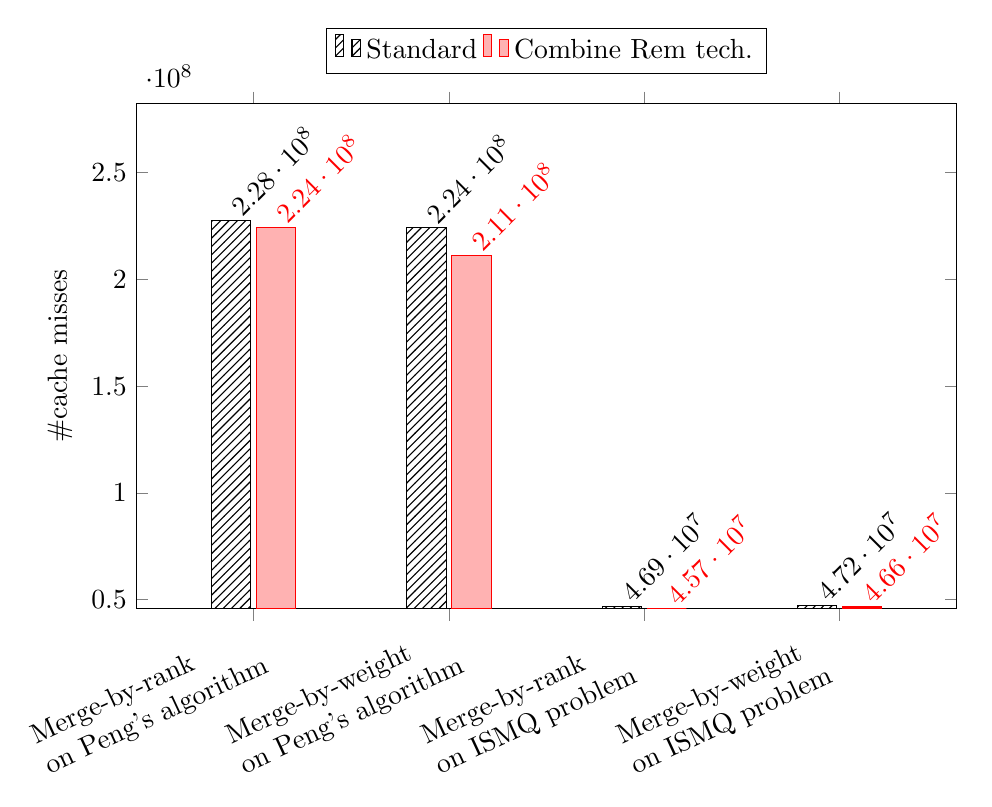
\begin{tikzpicture}
  \centering
  \begin{axis}[
  	bar width=0.5cm,
    ybar,
    xtick=\empty,
    enlargelimits=0.20,
    legend style={at={(0.5,1.15)},
    anchor=north,legend columns=-1},
    ylabel={\#cache misses},
    symbolic x coords={VGLCS Rank,VGLCS Weight, ISMQ Rank, ISMQ Weight},
    xtick={VGLCS Rank,VGLCS Weight, ISMQ Rank, ISMQ Weight},
    height=8cm,width=12cm,
    nodes near coords,
    nodes near coords align={vertical},
    every node near coord/.append style={
        anchor=mid west,
        rotate=45
    },
    xticklabel style={
	    inner sep=0pt,
	    anchor=north east,
	    rotate=25,
	    % font=\scshape,
        text width=9em
    },
    enlarge y limits={upper,value=0.3},
    xticklabels={
        Merge-by-rank \\on Peng's algorithm,
        Merge-by-weight \\on Peng's algorithm,
        Merge-by-rank \\on ISMQ problem,
        Merge-by-weight \\on ISMQ problem,
    },
    ]
    \addplot[pattern=north east lines] coordinates 
    	{(VGLCS Rank,227702431) (VGLCS Weight,224092655)
    	 (ISMQ Rank,46850580) (ISMQ Weight,47221311)
    	};
    \addplot coordinates 
    	{(VGLCS Rank,224163241) (VGLCS Weight,211097834)
    	 (ISMQ Rank,45720978) (ISMQ Weight,46577202)
    	};
    \legend{Standard, Combine Rem tech.};
  \end{axis}
\end{tikzpicture}

\end{document}
